\section{Experiments} 
 \subsection{Experimental setup}
  \begin{frame}
   \frametitle{Experimental setup}
   
   \begin{itemize}
    \item<1-> Use the three implemented networks and change the recurrent layer with PredRNN to see if this achieves better performance
    \item<2-> Experiments were performed on three different datasets
    \begin{itemize}
     \item<3-> MovingMNIST (synthetic dataset)
     \begin{itemize}
      \item<4-> Pre-processed to have frame size $(1 \times 64 \times 64)$, two digits per frame
      \item<5-> Training set of $10000$ sequences, with every sequence consisting of ten images
      \item<6-> Test set of $3000$ sequences
     \end{itemize}
     \item<7-> KTH (real dataset, fixed camera)
     \begin{itemize}
      \item<8-> Pre-processed to gray-scaled images, cropped to size $(1 \times 80 \times 60)$
     \end{itemize}
     \item<9-> Kitti (real dataset, ego-centric movement)
     \begin{itemize}
      \item<10-> Cropped to frame size $(3 \times 160 \times 128)$
     \end{itemize}
    \end{itemize}
   \end{itemize}

  \end{frame}
  \begin{frame}
   \frametitle{Experimental setup}
   
   \begin{itemize}
    \item<1-> First experiments were performed using fixed hyperparameter (HP optimization is only applied in the second experiments)
    \begin{itemize}
     \item<2-> In total $18$ different networks trained
     \item<3-> On own Computer $\Rightarrow$ Kitti training took $>12$h
    \end{itemize}
    \item<4-> MovingMNIST $5000$ iterations per epoch in one epoch (Inspired by Elsayed et al. \cite{Elsayed2018})
    \item<5-> KTH $500$ iterations per epoch in $20$ epochs
    \item<6-> Kitti $500$ iterations per epoch in $50$ epochs
    \item<7-> Adam \cite{Kingma2015} was used as optimizer with lr of $0.001$ and lr-scheduler reducing the lr after $\frac{epochs}{2}$ by factor ten
    \item<8-> Other hyperparamter can be found in the yml-folder of the implementation
   \end{itemize}      
   
  \end{frame}
  \begin{frame}
   \frametitle{Experimental setup}
   
   \begin{itemize}
    \item<1-> Second experiments are performed using HP optimization, using early-stopping and with \glqq optimal values\grqq
    \item<2-> Only one out of $18$ experiments performed, to get the importance of HP optimization and a tendency of how the results should look using optimal 
    conditions
   \end{itemize}
   
  \end{frame}
  
 \subsection{Experimental results (First setup)}
  \begin{frame}
   \frametitle{Experimental results (First setup)}
   
   \begin{itemize}
    \item<1-> Section is splitted into the three different datasets
    \item<2-> First comparison of trainable parameter amount
    \item<3-> Secondly table of mean MSE for testing and some example output
   \end{itemize}
  \end{frame}   
 
  \begin{frame}
   \frametitle{MovingMNIST}
   
   \begin{table}[H]
    \begin{center}
     \begin{tabular}{| l | l | l |}\hline
      \textbf{Model} & \textbf{ConvLSTM} & \textbf{PredRNN} \\\hline
      Autoencoder (Depth $2$) & $537.411$ & $773.018$ \\\hline
      PredNet & $6.909.818$ & $12.421.090$ \\\hline
      Spatiotemp & $1.001.324$ & $1.415.639$ \\\hline
     \end{tabular}
    \end{center}
    \caption{Number of trainable parameter for MovingMNIST.}
   \end{table}
   
  \end{frame}
  \begin{frame}
   \frametitle{MovingMNIST}
   
   \begin{figure}[H]
    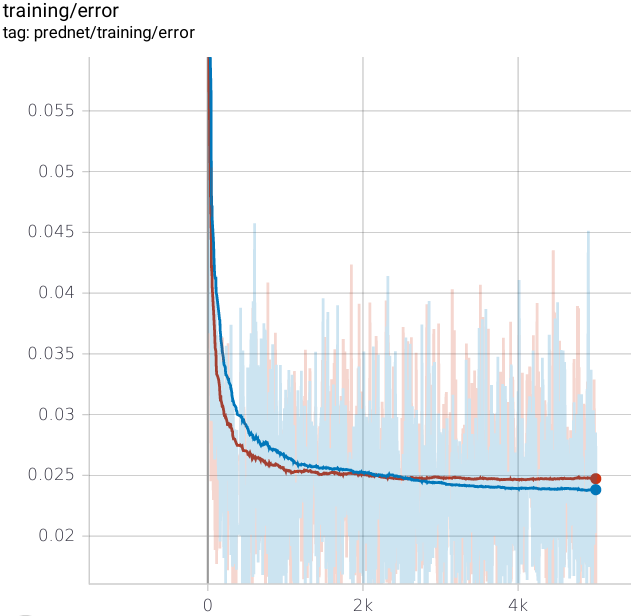
\includegraphics[width=0.45\textwidth]{../Images/prednet_mnist_training.png}
    \centering
    \caption{Training PredNet with ConvLSTM (blue) and PredRNN (red) on MovingMNIST.}
    \label{fig:prednet_mnist_training}
   \end{figure}
   
  \end{frame}
  \begin{frame}
   \frametitle{MovingMNIST}
   
   \begin{figure}[H]
   \centering
   \subfloat[Ground truth]{{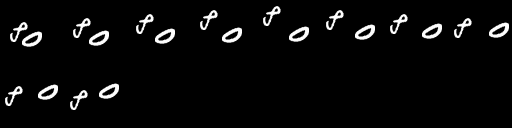
\includegraphics[width=0.6\textwidth]{../Images/prednet_mnist_groundtruth.png} }} 
   \qquad
   \subfloat[ConvLSTM]{{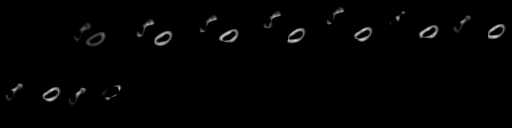
\includegraphics[width=0.6\textwidth]{../Images/prednet_mnist_convlstm_prediction.png} }} 
   \qquad
   \subfloat[PredRNN (vanished)]{{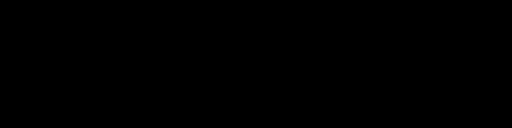
\includegraphics[width=0.6\textwidth]{../Images/prednet_mnist_predrnn_prediction.png} }}
   \caption{Test results for PredNet on MovingMNIST.}
   \label{figure::prednet_mnist_results} 
   \end{figure}
   
  \end{frame} 
  \begin{frame}
   \frametitle{MovingMNIST}
   
   \begin{table}[H]
    \begin{center}
     \begin{tabular}{| l | l | l |}\hline
      \textbf{Model} & \textbf{ConvLSTM} & \textbf{PredRNN} \\\hline
      Autoencoder (Depth $2$) & $0.027$ & $0.028$ \\\hline
      PredNet & $0.035$ & $0.041$ \\\hline
      Spatiotemp & $0.024$ & $0.022$ \\\hline
     \end{tabular}
    \end{center}
    \caption{Mean MSE for MovingMNIST.}
   \end{table}
   
  \end{frame}
  \begin{frame}
   \frametitle{KTH}
   
   \begin{table}[H]
    \begin{center}
     \begin{tabular}{| l | l | l |}\hline
      \textbf{Model} & \textbf{ConvLSTM} & \textbf{PredRNN} \\\hline
      Autoencoder (Depth $2$) & $542.531$ & $781.760$ \\\hline
      PredNet & $850.325$ & $1.285.730$ \\\hline
      Spatiotemp & $1.007.598$ & $1.421.913$ \\\hline
     \end{tabular}
    \end{center}
    \caption{Number of trainable parameter for KTH.}
   \end{table}
   
  \end{frame}
  \begin{frame}
   \frametitle{KTH}
   
   \begin{figure}[H]
   \centering
   \subfloat[Ground truth]{{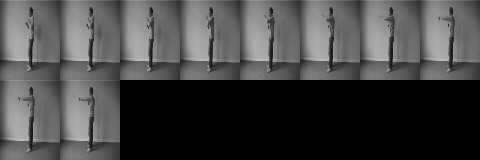
\includegraphics[width=0.45\textwidth]{../Images/prednet_kth_groundtruth.png} }} 
   \qquad
   \subfloat[ConvLSTM]{{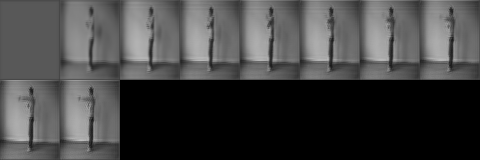
\includegraphics[width=0.45\textwidth]{../Images/prednet_kth_convlstm.png} }} 
   \qquad
   \subfloat[PredRNN]{{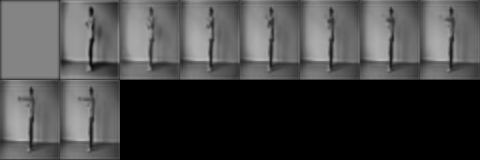
\includegraphics[width=0.45\textwidth]{../Images/prednet_kth_predrnn.png} }}
   \caption{Test results for PredNet on KTH.}
   \label{figure::prednet_kth_results}
  \end{figure}
  
  \end{frame}
  \begin{frame}
   \frametitle{KTH}
   
   \begin{table}[H]
    \begin{center}
     \begin{tabular}{| l | l | l |}\hline
      \textbf{Model} & \textbf{ConvLSTM} & \textbf{PredRNN} \\\hline
      Autoencoder (Depth $2$) & $1.55e-3$ & $0.05$ (didn't converged) \\\hline
      PredNet & $1.95e-3$ & $1.93e-3$ \\\hline
      Spatiotemp & $3.1e-3$ & $0.025$ (didn't converged) \\\hline
     \end{tabular}
    \end{center}
    \caption{Mean MSE for KTH.}
   \end{table}  
   
  \end{frame}
  \begin{frame}
   \frametitle{Kitti}
   
   \begin{table}[H]
    \begin{center}
     \begin{tabular}{| l | l | l |}\hline
      \textbf{Model} & \textbf{ConvLSTM} & \textbf{PredRNN} \\\hline
      Autoencoder (Depth $2$) & $542.531$ & $781.760$ \\\hline
      PredNet & $8.222.559$ & $12.430.626$ \\\hline
      Spatiotemp & $1.640.321$ & $2.200.641$ \\\hline
     \end{tabular}
    \end{center}
    \caption{Number of trainable parameter for Kitti.}
   \end{table} 
   
  \end{frame}
  \begin{frame}
   \frametitle{Kitti}
   
   \begin{figure}[H]
   \centering
   \subfloat[Ground truth]{{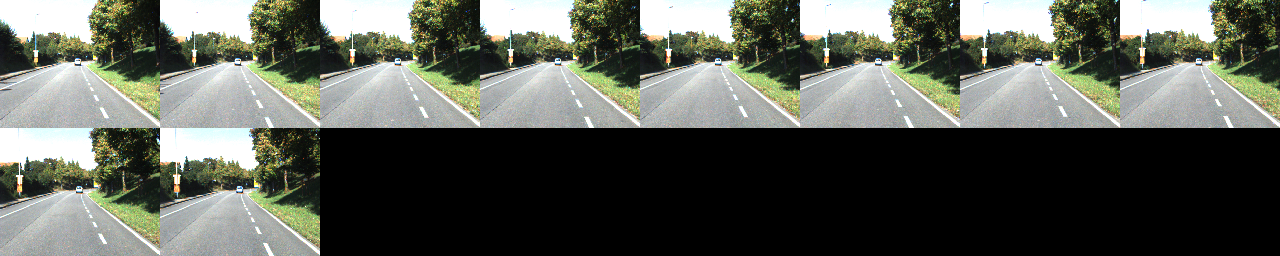
\includegraphics[width=0.7\textwidth]{../Images/prednet_kitti_groundtruth.png} }} 
   \qquad
   \subfloat[ConvLSTM]{{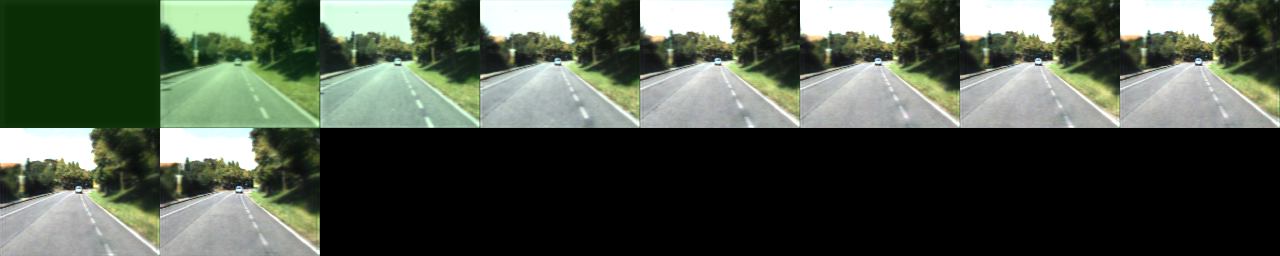
\includegraphics[width=0.7\textwidth]{../Images/prednet_kitti_convlstm.png} }} 
   \qquad
   \subfloat[PredRNN]{{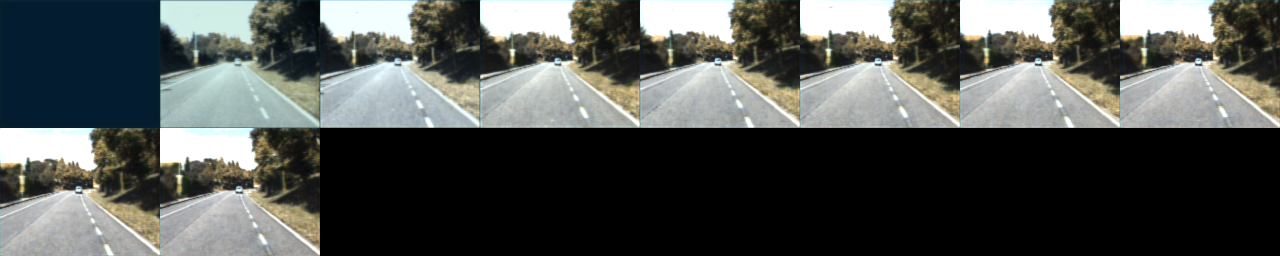
\includegraphics[width=0.7\textwidth]{../Images/prednet_kitti_predrnn.png} }}
   \caption{Test results for PredNet on Kitti.}
   \label{figure::prednet_kth_results}
  \end{figure}
   
  \end{frame}
  \begin{frame}
   \frametitle{Kitti}
   
   \begin{table}[H]
    \begin{center}
     \begin{tabular}{| l | l | l |}\hline
      \textbf{Model} & \textbf{ConvLSTM} & \textbf{PredRNN} \\\hline
      Autoencoder (Depth $2$) & $0.02$ & $0.013$ \\\hline
      PredNet & $0.019$ & $0.02$ \\\hline
      Spatiotemp & $0.018$ & $0.017$ \\\hline
     \end{tabular}
    \end{center}
    \caption{Mean MSE for Kitti.}
   \end{table}   
   
  \end{frame}
 
 \subsection{Experimental Results (Second setup)}
  \begin{frame}
   \frametitle{Experimental Results (Second setup)}
   
   \begin{itemize}
    \item<1-> Performed on KTH dataset with optimal values and lr of $0.0001$
   \end{itemize}
   
   \begin{figure}[H]
   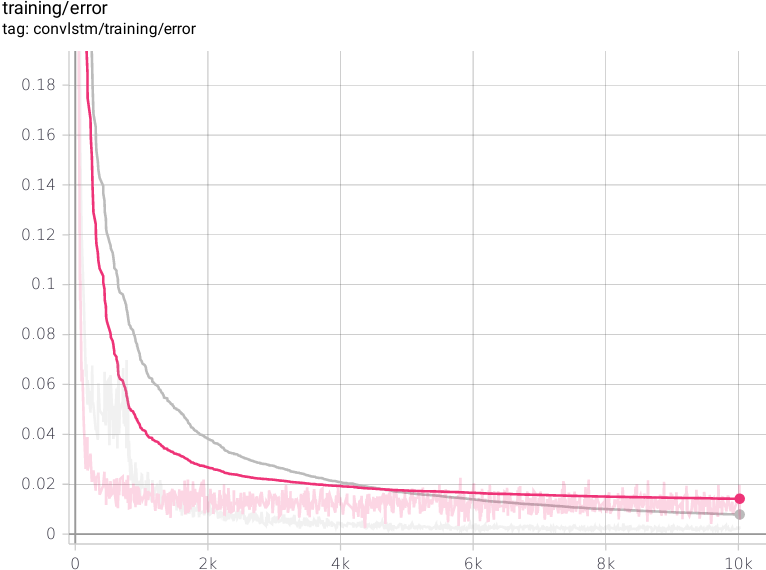
\includegraphics[width=0.6\textwidth]{../Images/exp2_training_error.png}
   \centering
   \caption{Training Autoencoder with ConvLSTM (red) and PredRNN (gray) on KTH using hyperparameter optimization and early stopping.}
   \label{fig:autoenc_exp2_training}
  \end{figure}   
   
  \end{frame}
  \begin{frame}
   \frametitle{Experimental Results (Second setup)}
   
   \begin{itemize}
    \item<1-> Mean test MSE for Autoencoder using ConvLSTM: \textbf{$0.0013$}
    \item<2-> Mean test MSE for Autoencoder using PredRNN: \textbf{$0.00072$}
    \item<3-> PredRNN is able to boost Autoencoder by more then $80$ percent
    \item<4-> Showed importance of HP optimization and early stopping
    \item<5-> Gives a hint of how the other experiments should perform
   \end{itemize}
  \end{frame}
  \begin{frame}
   \frametitle{Experimental Results (Second setup)}
   
   \begin{figure}[H]
   \centering
   \subfloat[Ground truth]{{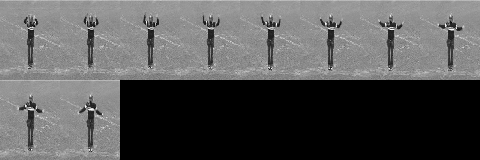
\includegraphics[width=0.65\textwidth]{../Images/exp2_test_ground.png} }} 
   \qquad
   \subfloat[ConvLSTM]{{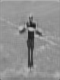
\includegraphics[width=0.1\textwidth]{../Images/exp2_test_convlstm.png} }} 
   \qquad
   \subfloat[PredRNN]{{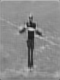
\includegraphics[width=0.1\textwidth]{../Images/exp2_test_predrnn.png} }}
   \caption{Test results for Autoencoder on KTH using hyperparameter optimization and early stopping.}
   \label{figure::prednet_mnist_results}
  \end{figure}
  
  \end{frame}